\documentclass[a4paper]{ctexart}
\usepackage{amsmath}
\usepackage{amsfonts}
\usepackage{amssymb}
\usepackage{amsthm}
\usepackage{bm}
\usepackage{graphicx}
\usepackage{textcomp}
\usepackage{url}
\usepackage[colorlinks,urlcolor=blue]{hyperref}
\usepackage[left=3cm, right=3cm]{geometry}
\DeclareMathOperator*{\argmax}{arg\,max}
\DeclareMathOperator*{\argmin}{arg\,min}

\title{\textbf{掼蛋AI系统开发文档}}
\author{陈钦霖\ 黄奕诚\ 赵士轩\ 王煜凯}
\date{\today}

\begin{document}

\maketitle

\section{简介}
我们完成了一个基于客户端-服务端架构的掼蛋AI系统。
该系统的源代码和使用方法已上传到\texttt{github}的仓库上\cite{guandan-ai}。
本文档主要描述系统的设计和实现。如果有其它任何疑惑,欢迎到项目主页进一步查阅。

首先,我们简单介绍一下客户端和服务端的功能。
想象一下我们自己在某个线上打牌系统打牌的时候,
我们仅需考虑轮到我们出牌的时候出什么牌,而剩下的工作都交给软件去处理。
这是一个很自然的过程。因此,我们的掼蛋AI系统也是这么设计的。

服务端和代表四个参与者的客户端进行通讯。
服务端负责告诉客户端``你有什么牌''、``别人出了什么牌''、``轮到你出牌了''等等,
并且把当前出牌的结果显示在GUI上。
客户端只需要在接收到服务端的消息后回应自己出的牌。
客户端出牌可以采用随机策略出牌,也可以采取智能的策略出牌,这取决于实现在客户端中AI算法的好坏。
客户端和服务端的架构带来的好处是,我们的AI算法与其它系统部件解耦,使得实现更加可控可分工。

该系统的UI如图\ref{fig:ui}所示。
图中有一个代表服务端的GUI和代表四个客户端的终端。
服务端上显示了当前牌局的进行情况,而客户端上打印了当前回合它所代表的参与者出的牌。

下面我们对服务端和客户端做更详细的介绍。
第\ref{sec:server}节主要描述了服务端的通讯协议,
然后第\ref{sec:client}节描述了客户端的实现细节以及我们实现在客户端中的AI算法。
为了验证我们AI算法的性能,我们还在第\ref{sec:experiment}节做了实验与各类基础策略进行比较。

\begin{figure}
  \centering
  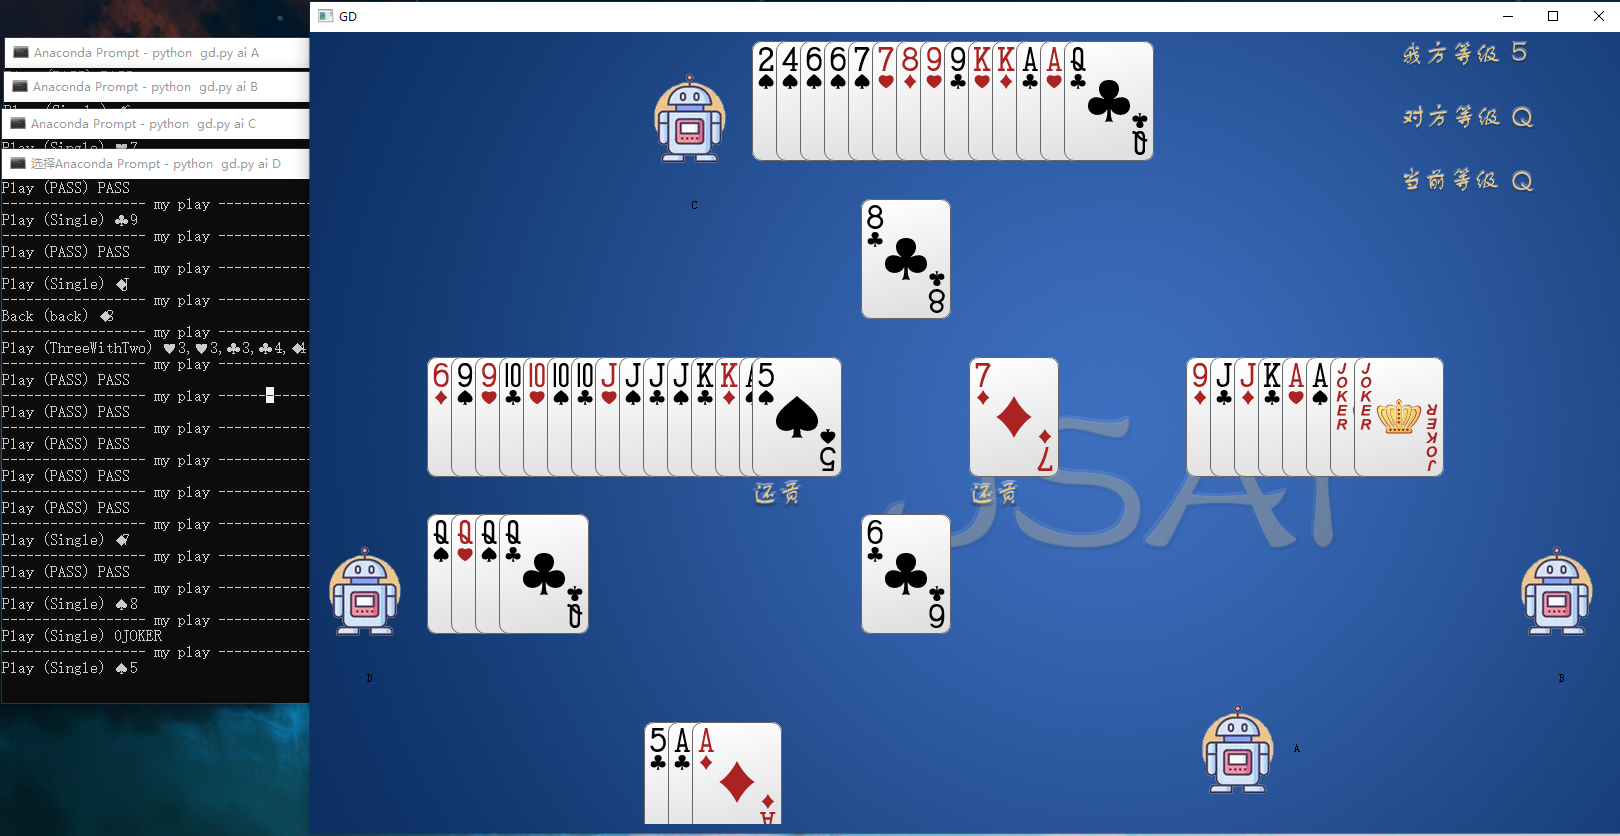
\includegraphics[width=\linewidth]{images/ui}
  \caption{掼蛋AI系统UI}
  \label{fig:ui}
\end{figure}

\section{服务端} \label{sec:server}
我们掼蛋AI系统的服务端主要负责下面两项任务:
\begin{enumerate}
  \item 告知客户端发生的事件 (例如:他人出牌、自己出牌、游戏结束),然后等待客户端做出选择
  (例如:在他人出牌时无需等待客户端做出选择,但在客户端出牌时需要等待客户端告知出什么牌)。
  \item 把事件的结果显示在GUI上(例如:当前每个玩家的手牌、当前牌桌上打出的牌、当前等级)。
\end{enumerate}

目前已经有了类似的服务端实现\cite{jsai}完成了这两项任务。
为了不重复造轮子,以便把更多精力放在AI算法上,我们以此为基础作为我们的服务端。
服务端的设计和实现细节可以从参考文献中的项目主页\cite{jsai}中进一步了解。
但是我们在介绍客户端的时候有用到协议相关的背景知识,
所以为了文档的完整性,我们仍需要简单介绍一下服务端和客户端的通讯协议。

\subsection{通讯协议} \label{subset:protocal}
服务端和客户端通过\texttt{websocket}传递JSON格式的消息进行通讯。
当客户端连接上服务端后,服务端会给客户端发送5种可能的消息,它们分别对应了5种事件的产生。
具体来说,消息类型被编码在了JSON对象的\texttt{type}字段里,有以下消息:
\begin{enumerate}
  \item 游戏结束消息(\texttt{type=0}):
  表示当客户端收到该消息时游戏已经结束。
  此消息还包含了一些其它字段用来表示一些重要的信息,其中包含出完牌的顺序和当前等级。
  客户端不需要回复该消息。
  
  \item 他人出牌消息(\texttt{type=1}):
  服务端通知客户端其它人打出的牌。
  该消息除了告知其它人打出的牌,还包含了很多其它重要的信息,
  其中包括当前客户端可出的牌、当前客户端的手牌、牌桌上的牌、其它人剩余的手牌数量等等。
  客户端不需要回复该消息。
  
  \item 自己出牌消息(\texttt{type=2,5,6}):
  服务端通知某客户端轮到它打出手牌。
  消息的其它字段和他人出牌消息一样。
  客户端需要回复该消息来回答服务端自己要出什么牌。
  \texttt{type=2,5,6}分别对应了普通出牌、进贡、还供三种不同的出牌情境。
\end{enumerate}

通讯协议的更多内容可以查询服务端项目网站\cite{jsai}上的文档来获得,
其它不必要的细节此处就不再赘述了。

\section{客户端} \label{sec:client}
\subsection{设计}
客户端的目标是完成与服务端通讯并在出牌阶段根据策略选择手牌打出。
为了在实验的时候对比使用不同策略的客户端,
我们需要把与服务器通讯的模块与策略模块解耦开来,减少代码的重复。

为了做到这一点,我们使用继承的机制。
我们有一个基类客户端,被称为\texttt{BaseClient},以及四个派生自基类的策略客户端,
分别被称为\texttt{RandomClient}、\texttt{MinClient}、texttt{HumanClient}和\texttt{AIClient}。

\subsubsection{基类客户端}
\texttt{BaseClient}首先完成与服务端的通讯功能。
它接受来自服务端的消息,并调用派生自它的客户端提供的回调方法处理消息,最后把结果封装重新发给服务端。

所有派生自它的客户端必须实现三个回调方法:
\begin{verbatim}
    finish(self, env)
    others_play(self, env)
    my_play(self, env)
\end{verbatim}
其中,派生客户端可以从\texttt{env}变量中获取从服务端发来的消息里的字段。
这三个方法分别被用来处理第\ref{subset:protocal}节中描述的5种消息,
具体来说,当游戏结束消息到来后,
\texttt{BaseClient}会把消息中的字段保存进\texttt{env}变量中,然后调用\texttt{finish(env)}。
当他人出牌消息到来后,\texttt{BaseClient}同样地会调用\texttt{others\_play(env)}。
当自己出牌消息到来后,\texttt{BaseClient}会调用\texttt{my\_play(env)}。
\texttt{my\_play(env)}必须返回一个手牌对象用来表示这轮你打出的手牌,
然后\texttt{BaseClient}把结果封装成协议规定的格式送给服务端。

\texttt{BaseClient}其次完成记忆功能。
就像我们打牌时会记牌一样,它也会提取并记录所收到的消息中有用的信息,
方便派生的策略客户端在打牌时查询、搜索、推理。
所有的记忆都可以通过\texttt{env}变量提供的接口提取。

\subsubsection{策略客户端}
我们总共实现了四个策略客户端。它们的策略如下:
\begin{enumerate}
  \item
  \texttt{RandomClient}:从可行的出牌中随机选择一种打出。

  \item
  \texttt{MinClient}:从可行的出牌中选择一种最小的打出。

  \item
  \texttt{HumanClient}:从命令行中读取人类的输入选择手牌打出。

  \item 
  \texttt{AIClient}:根据第\ref{subsec:ai-alg}节描述的策略选择手牌打出。
\end{enumerate}

\subsection{AI算法} \label{subsec:ai-alg}
目前,我们采用基于启发式策略的AI算法,其核心是自己出牌阶段的启发式规则。

在自己出牌时,根据牌权是否在自己手中能划分出两种情况:
\begin{enumerate}
  \item 牌权在自己。此时,按照优先级从高到低的顺序采取以下策略:
  \begin{enumerate}
    \item 大概率获胜策略:
    如果通过某种搜索或者推理的方法发现有一个出牌序列能使自己大概率获胜,
    那么按照这个能获胜的策略打出手牌。

    \item 辅助对家逃牌策略:
    如果对家还剩少量手牌(如不超过两张),而自己还剩很多牌,那么我们就要辅助对家逃牌。

    \item 逃牌策略:
    为了尽可能逃牌,选择出不少于五张的非炸弹牌型。

    \item 打击敌家策略:
    如果发现敌家只剩少量牌(如不超过两张),那么尽量出大少于三张的牌型。

    \item 最小策略:
    选择当前能出的最小的牌型。
  \end{enumerate}
  如果根据优先级高的策略没有合适的牌能打出,那么就依次选择优先级较低的策略。

  \item 没有牌权。此时,按照优先级从高到低的顺序采取以下策略:
  \begin{enumerate}
    \item 辅助对家策略:
    当对家出的牌大于某个阈值时(如炸弹,小王),放弃出牌。

    \item 跟牌策略:
    这里,我们采取一些形式化的方法来描述我们的策略。

    首先我们给出一些术语的定义。
    我们把\textbf{手牌}看作是牌的集合。
    给定一副手牌$H$,我们定义\textbf{拆牌}$P(H)$为$H$的划分(partition),
    并且满足对任意$a \in P(H)$,$a$都是一个满足掼蛋规则的牌型。
    在$H$明确的情况下,我们简记$P(H)$为$P$。
    对于一个拆牌$P$,若能把它进一步划分,得到新的拆牌$P'$,
    则称$P'$是$P$的\textbf{子拆牌}。
    举例来说,若某个拆牌$P$中有炸弹$a$,我们把炸弹拆成两个对子$a',a''$,
    就能得到子拆牌$P'=P\backslash\{a\}\cup\{a',a''\}$。
    假设当前能出的牌的集合是$A$,
    我们定义拆牌$P$是\textbf{有效拆牌}当且仅当$P\cap A\neq \emptyset$。
 
    我们希望能把牌拆成比较好的形式,使得按照拆牌中的牌型出牌能让我们有更大的可能获得胜利,
    就像我们一般不会把炸弹拆成对子,但我们会把对子拆成单张。
    所以我们定义一个\textbf{估值函数}$f$,它会把一个拆牌映射到实数上,代表此拆牌的价值。
    价值越高,就代表我们认为它更有可能带来胜利。
    准确反映胜率的估值函数一般很难计算得到,所以我们的估值函数一般是由启发策略定义的。
    比如,我们对拆牌中的每个牌型估分然后加总,就能得到一个估值。
    有了估值函数$f$后,给定一副手牌$H$,
    我们可以定义它的\textbf{最优拆牌}$P^*=\argmax_{P} f(P)$。
    
    最后,我们的跟牌策略如下。
    给定手牌$H$,当前可出的牌的集合$A$,以及估值函数$f$,设$P^*$是最优拆牌。
    若$P^*$中有与此轮出牌牌型一致的牌,那么打出最小的那个。
    否则,$P^*\cap A$为火牌 (炸弹、同花顺),或者空集。
    这种情况下,那么我们在一定深度内搜索$P^*$的最优有效子拆牌$P'$。
    若$P'$不存在或$f(P')$远小于$f(P^*)$,
    那么我们放弃$P'$,根据对家牌面的大小从$P^*$中选择火牌或不出。
    否则,我们从$P'\cap A$选择一张最小能出的牌打出。
    
    这里举个例子。
    如果敌家出了44,而你只可能出炸弹5555,或相对最优地,你也可以把它拆成两个55来压敌家。
    但炸弹估值很高,而单张、一对和三张的估值都较低,如果拆了炸弹,那么估值的损失就会很大,这是无法接受的。
    所以根据我们的策略,要么直接炸,要么PASS。
    但如果你最优拆牌是55444,里面没有与44一致的牌型,
    但把55444拆成55+444,估值并不会怎么下降(因为444可以跟很多其它牌搭),
    这时根据我们的策略就会打出55。
    
  \end{enumerate}
\end{enumerate}

\section{实验} \label{sec:experiment}


\begin{thebibliography}{99}
  \bibitem{guandan-ai}
  \url{https://github.com/QinlinChen/guandan-ai}

  \bibitem{jsai}
  \url{http://www.jsai-gd.com/}
\end{thebibliography}
\end{document}